\section{Paper 3}

\title[PhD Defence]{
    {\Huge Paper 3} \\
    \vspace{2mm}
    {\Large \tool{}: Scalable Analysis of Weakly-Hard Constraints} \\
}
\author[Nils Vreman]{
    Nils Vreman \\
    \vspace{3mm}
    {\large Richard Pates, Martina Maggio}
}
\date[RTAS 2022]{
    Real-Time and Embedded Technology and Applications Symposium, 2022\\
    {\large RTAS Artifact Evaluation - Passed}
}
\notitlelogo
\frame[plain,noframenumbering]{\titlepage}


\begin{frame}
    \frametitle{The Weakly-Hard Model}
    \begin{minipage}[c]{0.24\textwidth}
        \centering
        \begin{equation*}
            \begin{matrix}
                {\Large \anyhit{}}   \\
                            \\
                \tAH{}
            \end{matrix}
        \end{equation*}
    \end{minipage}\hfill
    \begin{minipage}[c]{0.24\textwidth}
        \centering
        \begin{equation*}
            \begin{matrix}
                {\Large \anymiss{}}   \\
                            \\
                \tAM{}
            \end{matrix}
        \end{equation*}
    \end{minipage}\hfill
    \begin{minipage}[c]{0.24\textwidth}
        \centering
        \begin{equation*}
            \begin{matrix}
                {\Large \rowhit{}}   \\
                            \\
                \tRH{}
            \end{matrix}
        \end{equation*}
    \end{minipage}\hfill
    \begin{minipage}[c]{0.24\textwidth}
        \centering
        \begin{equation*}
            \begin{matrix}
                {\Large \rowmiss{}}   \\
                            \\
                \tRM{}
            \end{matrix}
        \end{equation*}
    \end{minipage}

    \vspace{1cm}

    \begin{equation*}
        \ldots\, 0\, 1\, 1\, 1\, 0\, 1\, 0\, 1\, 1\, 1\, 0\, 0\, 1\, 1\, 1\, 0\, 1\, 0\, 1\, 1\, 0\, 0\, 1\, 1\, 0\, 1\, 1\, 0\, 1\, 1\, 1\, 1\, 1\, 0\, \ldots
    \end{equation*}
\end{frame}


\begin{frame}
    \frametitle{The Weakly-Hard Model}

    \begin{itemize}\setlength\itemsep{1em}
        \item Historically: Focus on $\tAM{}$ $\anymiss{}$
        \item $\tRH{}$ $\rowhit{}$ better motivated by control problems\footnote{\cite{Linsenmayer:2021,Vreman:2021}}
            \begin{itemize}
                \item \textbf{Paper 3}: Two new theorems
            \end{itemize}
        \item No joint framework for analysing the weakly-hard models
            \begin{itemize}
                \item \textbf{Paper 3}: \tool{}
            \end{itemize}
    \end{itemize}
\end{frame}


\begin{frame}
    \frametitle{The Weakly-Hard Model}
    \framesubtitle{Relations}
    \begin{figure}[h]
        \centering
        \only<1>{\begin{tikzpicture}
    \draw[dashed, thick, gray] (1,0) grid[xstep=2, ystep=1.25] (10,6);

    \node[anchor=east] at (1.75, 4.375) {\tAH\, $\binom{a}{b}$};
    \node[anchor=east] at (1.75, 3.125) {\tAM\, $\overline{\binom{a}{b}}$};
    \node[anchor=east] at (1.75, 1.875) {\tRH\, $\genfrac{<}{>}{0pt}{}{a}{b}$};
    \node[anchor=east] at (1.75, 0.625) {\tRM\, $\overline{\genfrac{<}{>}{0pt}{}{a}{b}}$};

    \node[anchor=south] at (3, 5.25) {$\binom{c}{d}$};
    \node[anchor=south] at (5, 5.25) {$\overline{\binom{c}{d}}$};
    \node[anchor=south] at (7, 5.25) {$\genfrac{<}{>}{0pt}{}{c}{d}$};
    \node[anchor=south] at (9, 5.25) {$\overline{\genfrac{<}{>}{0pt}{}{c}{d}}$};

    % AnyHit
    \node at (3, 4.375) {\footnotesize $\preceq$};
    \node at (5, 4.375) {\footnotesize $\binom{a}{b} \equiv \overline{\binom{b-a}{b}}$};
    \node at (7, 4.375) {\footnotesize $\cdot$};
    \node at (9, 4.375) {\footnotesize $\overline{\genfrac{<}{>}{0pt}{}{c}{d}} \equiv \binom{1}{c+1}$};

    % AnyMiss
    \node at (3, 3.125) {\footnotesize $\overline{\binom{a}{b}} \equiv \binom{b-a}{b}$};
    \node at (5, 3.125) {\footnotesize $\preceq$};
    \node at (7, 3.125) {\footnotesize $\cdot$};
    \node at (9, 3.125) {\footnotesize $\overline{\genfrac{<}{>}{0pt}{}{c}{d}} \equiv \overline{\binom{c}{c+1}}$};

    % RowHit
    \node at (3, 1.875) {\footnotesize $\cdot$};
    \node at (5, 1.875) {\footnotesize $\cdot$};
    \node at (7, 1.875) {\footnotesize $\preceq$};
    \node at (9, 1.875) {\footnotesize $\cdot$};

    % RowMiss
    \node at (3, 0.625) {\footnotesize $\overline{\genfrac{<}{>}{0pt}{}{a}{b}} \equiv \binom{1}{a+1}$};
    \node at (5, 0.625) {\footnotesize $\overline{\genfrac{<}{>}{0pt}{}{a}{b}} \equiv \overline{\binom{a}{a+1}}$};
    \node at (7, 0.625) {\footnotesize $\cdot$};
    \node at (9, 0.625) {\footnotesize $\preceq$};

\end{tikzpicture}
}%
        \only<2>{\begin{tikzpicture}
    \draw[dashed, thick, gray] (1,0) grid[xstep=2, ystep=1.25] (10,6);

    \node[anchor=east] at (1.75, 4.375) {\tAH\, $\binom{a}{b}$};
    \node[anchor=east] at (1.75, 3.125) {\tAM\, $\overline{\binom{a}{b}}$};
    \node[anchor=east] at (1.75, 1.875) {\tRH\, $\genfrac{<}{>}{0pt}{}{a}{b}$};
    \node[anchor=east] at (1.75, 0.625) {\tRM\, $\overline{\genfrac{<}{>}{0pt}{}{a}{b}}$};

    \node[anchor=south] at (3, 5.25) {$\binom{c}{d}$};
    \node[anchor=south] at (5, 5.25) {$\overline{\binom{c}{d}}$};
    \node[anchor=south] at (7, 5.25) {$\genfrac{<}{>}{0pt}{}{c}{d}$};
    \node[anchor=south] at (9, 5.25) {$\overline{\genfrac{<}{>}{0pt}{}{c}{d}}$};

    % AnyHit
    \node at (3, 4.375) {\footnotesize $\preceq$};
    \node at (5, 4.375) {\footnotesize $\binom{a}{b} \equiv \overline{\binom{b-a}{b}}$};
    \node at (7, 4.375) {\footnotesize $\cdot$};
    \node at (9, 4.375) {\footnotesize $\overline{\genfrac{<}{>}{0pt}{}{c}{d}} \equiv \binom{1}{c+1}$};

    % AnyMiss
    \node at (3, 3.125) {\footnotesize $\overline{\binom{a}{b}} \equiv \binom{b-a}{b}$};
    \node at (5, 3.125) {\footnotesize $\preceq$};
    \node at (7, 3.125) {\footnotesize $\cdot$};
    \node at (9, 3.125) {\footnotesize $\overline{\genfrac{<}{>}{0pt}{}{c}{d}} \equiv \overline{\binom{c}{c+1}}$};

    % RowHit
    \node at (3, 1.875) {\footnotesize $\cdot$};
    \node at (5, 1.875) {\footnotesize $\cdot$};
    \node at (7, 1.875) {\footnotesize $\preceq$};
    \node at (9, 1.875) {\footnotesize $\cdot$};

    % RowMiss
    \node at (3, 0.625) {\footnotesize $\overline{\genfrac{<}{>}{0pt}{}{a}{b}} \equiv \binom{1}{a+1}$};
    \node at (5, 0.625) {\footnotesize $\overline{\genfrac{<}{>}{0pt}{}{a}{b}} \equiv \overline{\binom{a}{a+1}}$};
    \node at (7, 0.625) {\footnotesize $\cdot$};
    \node at (9, 0.625) {\footnotesize $\preceq$};

    {\color{hicolour}\node[draw, thick, fill=white, align=center] at (1, 5.5) {\small Relationship\\\small Operator};}
    {\color{hicolour}\draw[thick, -latex] (1, 4.975) -- (2.85, 4.375);}

\end{tikzpicture}
}%
        \only<3>{\begin{tikzpicture}
    \draw[dashed, thick, gray] (1,0) grid[xstep=2, ystep=1.25] (10,6);

    \node[anchor=east] at (1.75, 4.375) {\tAH\, $\binom{a}{b}$};
    \node[anchor=east] at (1.75, 3.125) {\tAM\, $\overline{\binom{a}{b}}$};
    \node[anchor=east] at (1.75, 1.875) {\tRH\, $\genfrac{<}{>}{0pt}{}{a}{b}$};
    \node[anchor=east] at (1.75, 0.625) {\tRM\, $\overline{\genfrac{<}{>}{0pt}{}{a}{b}}$};

    \node[anchor=south] at (3, 5.25) {$\binom{c}{d}$};
    \node[anchor=south] at (5, 5.25) {$\overline{\binom{c}{d}}$};
    \node[anchor=south] at (7, 5.25) {$\genfrac{<}{>}{0pt}{}{c}{d}$};
    \node[anchor=south] at (9, 5.25) {$\overline{\genfrac{<}{>}{0pt}{}{c}{d}}$};

    % AnyHit
    \node at (3, 4.375) {\footnotesize $\preceq$};
    \node at (5, 4.375) {\footnotesize $\binom{a}{b} \equiv \overline{\binom{b-a}{b}}$};
    \node at (7, 4.375) {\footnotesize \textcolor{blue}{$\binom{a}{b} \stackrel{?}{\preceq} \genfrac{<}{>}{0pt}{}{c}{d}$}};
    \node at (9, 4.375) {\footnotesize $\overline{\genfrac{<}{>}{0pt}{}{c}{d}} \equiv \binom{1}{c+1}$};

    % AnyMiss
    \node at (3, 3.125) {\footnotesize $\overline{\binom{a}{b}} \equiv \binom{b-a}{b}$};
    \node at (5, 3.125) {\footnotesize $\preceq$};
    \node at (7, 3.125) {\footnotesize $\cdot$};
    \node at (9, 3.125) {\footnotesize $\overline{\genfrac{<}{>}{0pt}{}{c}{d}} \equiv \overline{\binom{c}{c+1}}$};

    % RowHit
    \node at (3, 1.875) {\footnotesize \textcolor{blue}{$\genfrac{<}{>}{0pt}{}{a}{b} \stackrel{?}{\preceq} \binom{c}{d}$}};
    \node at (5, 1.875) {\footnotesize $\cdot$};
    \node at (7, 1.875) {\footnotesize $\preceq$};
    \node at (9, 1.875) {\footnotesize $\cdot$};

    % RowMiss
    \node at (3, 0.625) {\footnotesize $\overline{\genfrac{<}{>}{0pt}{}{a}{b}} \equiv \binom{1}{a+1}$};
    \node at (5, 0.625) {\footnotesize $\overline{\genfrac{<}{>}{0pt}{}{a}{b}} \equiv \overline{\binom{a}{a+1}}$};
    \node at (7, 0.625) {\footnotesize $\cdot$};
    \node at (9, 0.625) {\footnotesize $\preceq$};

    \node[draw, rectangle, align=center, ultra thick, fill=blue!30] at (7, 2.5) {Can we say something\\about the relation between two\\ \emph{generic} \tAH{} and \tRH{}\\constraints?};

\end{tikzpicture}
}%
        \only<4>{\begin{tikzpicture}
    \draw[dashed, thick, gray] (1,0) grid[xstep=2, ystep=1.25] (10,6);

    \node[anchor=east] at (1.75, 4.375) {\tAH\, $\binom{a}{b}$};
    \node[anchor=east] at (1.75, 3.125) {\tAM\, $\overline{\binom{a}{b}}$};
    \node[anchor=east] at (1.75, 1.875) {\tRH\, $\genfrac{<}{>}{0pt}{}{a}{b}$};
    \node[anchor=east] at (1.75, 0.625) {\tRM\, $\overline{\genfrac{<}{>}{0pt}{}{a}{b}}$};

    \node[anchor=south] at (3, 5.25) {$\binom{c}{d}$};
    \node[anchor=south] at (5, 5.25) {$\overline{\binom{c}{d}}$};
    \node[anchor=south] at (7, 5.25) {$\genfrac{<}{>}{0pt}{}{c}{d}$};
    \node[anchor=south] at (9, 5.25) {$\overline{\genfrac{<}{>}{0pt}{}{c}{d}}$};

    % AnyHit
    \node at (3, 4.375) {\footnotesize $\preceq$};
    \node at (5, 4.375) {\footnotesize $\binom{a}{b} \equiv \overline{\binom{b-a}{b}}$};
    \node at (7, 4.375) {\footnotesize \textcolor{hicolour}{$\binom{a}{b} \stackrel{!}{\preceq} \genfrac{<}{>}{0pt}{}{c}{d}$}};
    \node at (9, 4.375) {\footnotesize $\overline{\genfrac{<}{>}{0pt}{}{c}{d}} \equiv \binom{1}{c+1}$};

    % AnyMiss
    \node at (3, 3.125) {\footnotesize $\overline{\binom{a}{b}} \equiv \binom{b-a}{b}$};
    \node at (5, 3.125) {\footnotesize $\preceq$};
    \node at (7, 3.125) {\footnotesize $\cdot$};
    \node at (9, 3.125) {\footnotesize $\overline{\genfrac{<}{>}{0pt}{}{c}{d}} \equiv \overline{\binom{c}{c+1}}$};

    % RowHit
    \node at (3, 1.875) {\footnotesize \textcolor{hicolour}{$\genfrac{<}{>}{0pt}{}{a}{b} \stackrel{!}{\preceq} \binom{c}{d}$}};
    \node at (5, 1.875) {\footnotesize $\cdot$};
    \node at (7, 1.875) {\footnotesize $\preceq$};
    \node at (9, 1.875) {\footnotesize $\cdot$};

    % RowMiss
    \node at (3, 0.625) {\footnotesize $\overline{\genfrac{<}{>}{0pt}{}{a}{b}} \equiv \binom{1}{a+1}$};
    \node at (5, 0.625) {\footnotesize $\overline{\genfrac{<}{>}{0pt}{}{a}{b}} \equiv \overline{\binom{a}{a+1}}$};
    \node at (7, 0.625) {\footnotesize $\cdot$};
    \node at (9, 0.625) {\footnotesize $\preceq$};

\end{tikzpicture}
}
    \end{figure}
\end{frame}


\begin{frame}
    \frametitle{\tool{}}
    \framesubtitle{Automata}
    \begin{minipage}[c]{0.39\textwidth}
        {\Large

        \vspace{2cm}

        $\anyhit{} = \binom{1}{3}$

        \vspace{2cm}

        \visible<2->{\alert<2>{$\dots 0$}}
        \visible<3->{\textcolor<3>{lqgcolour}{$1$}}
        \visible<4->{\alert<4>{$0$}}
        \visible<5->{\alert<5>{$0$}}
        \visible<6->{\textcolor<6>{lqgcolour}{$1$}}
        \visible<7->{\textcolor<7>{lqgcolour}{$1$}}
        \visible<8->{\alert<8>{$0\dots$}}
        }
    \end{minipage}
    \begin{minipage}[c]{0.59\textwidth}
        \centering
        \begin{figure}[h]
            \begin{tikzpicture}[>=latex]
                \node[Init Node] (a) at (0,0) {$1$};
                \node[Dom Node] (b) at (0,-1.75) {$10$};
                \node[Dom Node] (c) at (0,-3.5) {$100$};
                \invisible<7>{\draw[->] (a) edge [loop above] node[above] {$1$} (a);}
                \invisible<2,4,8>{\draw[->] (a) edge [bend left=67.5] node[right] {$0$} (b);}
                \invisible<3>{\draw[->] (b) edge [bend left=50] node[right] {$1$} (a);}
                \invisible<5>{\draw[->] (b) edge [bend left=67.5] node[right] {$0$} (c);}
                \invisible<6>{\draw[->] (c) edge [bend left=57.5] node[left] {$1$} (a);}
                
                \only<7>{\draw[->, thick, lqgcolour] (a) edge [loop above] node[above] {$1$} (a);}
                \only<2,4,8>{\draw[->, thick, red] (a) edge [bend left=67.5] node[right] {$0$} (b);}
                \only<3>{\draw[->, thick, lqgcolour] (b) edge [bend left=50] node[right] {$1$} (a);}
                \only<5>{\draw[->, thick, red] (b) edge [bend left=67.5] node[right] {$0$} (c);}
                \only<6>{\draw[->, thick, lqgcolour] (c) edge [bend left=57.5] node[left] {$1$} (a);}
                \draw[white] (0,-3.5) rectangle (0.1,-4.5);
            \end{tikzpicture}
        \end{figure}
    \end{minipage}
\end{frame}


\begin{frame}
    \frametitle{\tool{}\footnote{Published to \texttt{JuliaRegistries}.}}
    \begin{figure}[h]
        \centering
        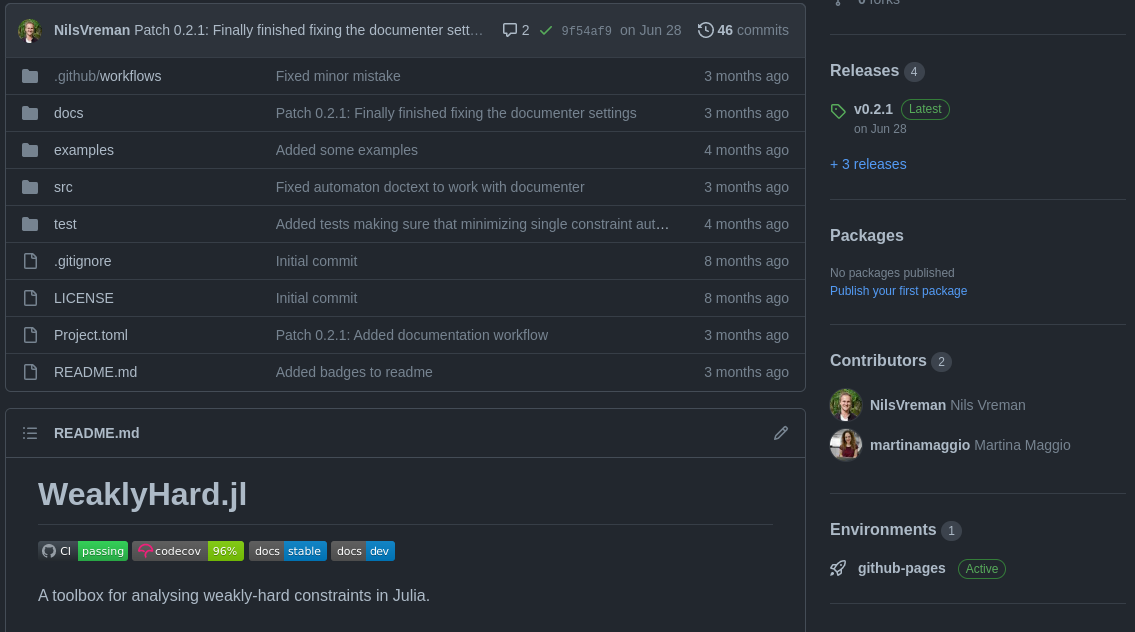
\includegraphics[width=0.7\textwidth]{figs/rtas22b/git.png}
    \end{figure}

    \begin{center}
        \Large
        \textcolor{blue}{\url{https://github.com/NilsVreman/WeaklyHard.jl}}
    \end{center}
\end{frame}

\begin{frame}
    \frametitle{\tool{}}
    \framesubtitle{Contribution}

    \begin{itemize}\setlength\itemsep{1em}
        \item Handle \emph{all} WH Constraints
        \item Handle \emph{sets} of WH Constraints
        \item Efficiently handle constraints with large windows $k$
    \end{itemize}
\end{frame}
